\chapter{Paulions and Gammions}
\label{ch-paulions}

\section{Paulions}

$\vec{a}\in\RR^3$

$\hat{a}= \frac{\vec{a}}{|
\vec{a}|}$

$i=1,2,3$, $\mu=0,1,2,3$

Pauli matrices

\beq
\s_x=\s_1=\left(
\begin{array}{cc}
0&1
\\
1&0
\end{array}
\right),\quad
\s_y=\s_2=\left(
\begin{array}{cc}
0&-i
\\
i&0
\end{array}
\right),\quad
\s_z=\s_3=\left(
\begin{array}{cc}
1&0
\\
0&-1
\end{array}
\right)
\eeq

Hermitian 

\beq
\s_i^\dagger = \s_i
\eeq

Square is 1 (unitary too  because Hermitian)
\beq 
\s_i^2 = 1
\eeq



\beq
\s_x \s_y= -\s_y \s_x 
\eeq
\beq
\s_x \s_y = i \s_z
\eeq

 \beq
\sigma_i \sigma_j = \delta_{ij} I_2+ i \epsilon_{ijk}\sigma_k
\eeq

\beq
\vec{\s}= (\s_1, \s_2, \s_3)
\eeq

\beq
\s_0=\left(
\begin{array}{cc}
1&0
\\
0&1
\end{array}
\right),\quad
\s_\mu = (\s_0, \vec{\s})
\eeq

Suppose $\vec{x}=(x_	1, x_2, x_3)\in\RR^3$. We define the 
{\bf Paulion} $\s_{\vec{x}}$ by\footnote{The term Paulion is not commonly used. As far as I know, $\s_{\vec{a}}$ doesn't
have a common name.}
\beq
\s_{\vec{x}} = \sigma\cdot \vec{x}=x_1\sigma_1 + x_2\sigma_2 + x_3\sigma_3
\eeq

\begin{claim}

\beq
\s_{\vec{a}}\s_{\vec{b}}=
\vec{a}\cdot\vec{b}+i\s_{\vec{a}\times\vec{b}}
\eeq

With $\vec{a}=\vec{b}$:

\beq
(\s_{\vec{a}})^2 = |\vec{a}|^2 
\eeq

With unit vector $\hat{a}$:
\beq
(\s_{\hat{a}})^2 = 1
\eeq
\end{claim}
\proof
\qed

\begin{claim}
If $\vec{a}\in \RR^3$ then

\beq
e^{i\s_{\vec{a}}}=
\cos |\vec{a}|
+
i \s_{\hat{a}}\sin |\vec{a}|
\eeq
and

\beq
U=e^{-i\frac{\theta}{2}\s_{\hat{a}}}=
\cos(\tfrac\theta2)-i\s_{\hat{a}}\sin(\tfrac\theta2)
\eeq
\end{claim}
\proof

\beq
e^{i
\theta \s_i}=
\cos \theta
+
i \s_i \sin \theta 
\eeq
\qed

\begin{figure}[h!]
\centering
\includegraphics[width=2.5in]
{paulions/Rx-pic.png}
\caption{Geometry of $R_{\hat{a}}(\theta)x$}
\label{fig-Rx-pic}
\end{figure}


\begin{claim}
\beq
U\s_{\vec{x}}U^\dagger
=
\sigma_{R_{\hat{a}}(\theta)\vec{x}}
\eeq
where

\beq
U=e^{-i\frac{\theta}{2}\s_{\hat{a}}}
\eeq

\beq
R_{\hat{a}}(\theta)\vec{x}=
\vec{x}
+(2|\vec{x}|\sin\beta\sin\theta)(-\sin\theta \hat{r}+
\cos\theta \hat{\theta})
\eeq
where (see Fig.\ref{fig-Rx-pic})

\beq
\beta=\angle(\vec{x}, \vec{a}),\quad
\hat{\theta}=
\frac{(\hat{a}\times\vec{x})}
{|\vec{x}|\sin\beta},\quad
\hat{r}=
\frac{[\vec{x}-\hat{a}(\hat{a}\cdot\vec{x})]}{|\vec{x}|\sin\beta}
\eeq
This immediately implies that
$SU(2)$ is a double cover of $SO(3)$.

\beq
SU(2)\xymatrix{\ar[r]_{\text{2 to 1 map}}&} SO(3),\quad SU(2)/\{1, -1\} \cong SO(3)\eeq
\end{claim}
\proof






If $U$ produces rotation $R$, then $-U$ gives the same rotation:

\beq
(-U) \s_{\vec{x}} (-U)^\dagger = U\s_{\vec{x}}U^\dagger.
\eeq

\qed


\begin{claim}
\beq
\s_{\vec{a}}\s_{\vec{x}}
\s_{\vec{a}}=
\sigma\cdot\left[
\vec{x}(2(\vec{a}\cdot\vec{a}) -1)
-2\vec{a}\times(\vec{a}\times\vec{x})
  \right]
\eeq
\end{claim}
\proof
\qed

\begin{claim}
\beq
-\s_{\hat{a}}\s_{\vec{x}}\s_{\hat{a}}=
\sigma_{\rho_{\hat{a}}\vec{x}}=\gamma_{\hat{\rva}}(\vec{x})
\eeq

\beq
\rho_{\hat{a}}\vec{x}=\vec{x} - 2(\hat{a}\cdot\vec{x})\hat{a}
\eeq


\



\end{claim}
\proof
\qed

\begin{claim}
\beq
[\s_{\vec{a}}, \s_{\vec{b}}]_+
= 2(\vec{a}\cdot\vec{b})
\eeq

\beq
[\s_{\vec{a}}, \s_{\vec{b}}]
= 2 i\s_{\vec{a}\times\vec{b}}
\eeq

\end{claim}
\proof
\qed





\section{Gammions}

\beq
a\cdot b= a_\mu b^\mu
\eeq

Suppose $a_\mu\in\RR$
for each $\mu$. We define
the {\bf Gammion} $\gamma_a$ by\footnote{The term Gammion, like the term Paulion, is not commonly used. As far as I know, $\gamma_a$ doesn't
have a common name.}


\beq
\gamma\cdot a = \gamma_\mu a^\mu = \gamma_a
\eeq


\beq
[\gamma_\mu,\gamma_\nu]_+=2\eta_{\mu\nu}
\eeq

with $\eta_{\mu\nu}$ equals Euclidean $(1,1,1,1)$ or Lorentzian $(1, -1,-1,-1)$ metric.


\beq
\gamma_a \gamma_b
= a\cdot b + i\gamma_{\mu\nu} a^\mu b^\nu,
\eeq
where bivector

\beq
\gamma_{\mu\nu}=-i\frac{1}{2}[\gamma_\mu,\gamma_\nu]
\eeq
is the generator of $\mathfrak{so}(n)$ or $\mathfrak{so}(p,q)$.


A rotation by  $\omega_{\mu\nu}$   is

\beq
S(\omega)=e^{-\;\frac{i}{4}\omega^{\mu\nu}\gamma_{\mu\nu}}
\eeq

\beq
 S \gamma_\rvx S^\dagger = \gamma_{Rx}
\eeq
where $R\in SO(n)$ (or $SO(p,q)$).
 
\section{$Spin(n)$}
\beq
Spin(n)=
\{e^{-\frac{i}{4}\omega^{\mu\nu}\gamma_{\mu\nu}}|
\omega_{\mu\nu}=-\omega_{\nu\mu}\in\RR
\}
\eeq


$n_-=n$ for $n$ even and $n_-=n-1$
for $n$ odd.

$e_i\in\RR^n$ for $i=1, 2, \ldots n$. All components
of $e_i$ are zero except the $i$th one.

\beq
\gamma_i=\gamma_{\rve_i}
\eeq

\beq
[\gamma_{i}, \gamma_{j}]_+ = 2 \delta_{i,j}
\eeq

\beq
\Pi_0 = \{1\},
\quad |\Pi_0|=1
\eeq

\beq
\Pi_1=\{\gamma_i|i=1, 2, \ldots, n\}
\quad |\Pi_1|={n\choose 1}=n
\eeq

\beq
\Pi_2=
\{ \gamma_{i_1}\gamma_{ i_2}|i_1<i_2 \},
\quad |\Pi_2|={n\choose 2}
\eeq

\beq
\Pi_3=
\{ \gamma_{i_1}\gamma_{ i_2}\gamma_{i_3}|i_1<i_2<i_3 \},
\quad |\Pi_3|={n\choose 3}
\eeq

\beq
\Pi_{2^n}=
\{\gamma_1\gamma_2\ldots\gamma_n\},
\quad |\Pi_{2^n}|={n\choose n}=1
\eeq

\beq
\sum_{k=0}^n {n\choose k}= (1+1)^n=2^n
\eeq

\beq
Cl(n)=span_\RR
\left(\bigcup_{k=0,1,2,\ldots, 2^n}\Pi_k
\right)
\eeq



\beq
Cl^0(n) = span_\RR
\left(\bigcup_{k=0,2,4,\ldots ,2^{n_-}}\Pi_k
\right)
\eeq

\beq
Cl^1(n) = span_\RR
\left(\bigcup_{k=1,3,5,\ldots ,2^{n_-}}\Pi_k
\right)
\eeq

\beq
Cl(n)= Cl^0(n) \oplus Cl^1(n)
\eeq

Since $S$ is the exponentiation of a bivector, its Taylor expansion only
contains summands with an even number 
of gammas.
\beq
Spin(n)
\subset Cl^0(n)
\eeq


\beq
 - \gamma_{\hat{\rva}} \gamma_{\rvx} \gamma_{\hat{\rva}}=
\gamma_{\ul{\rho_{\hat{a}}x}}=\gamma_{\hat{\rva}}(x)
\eeq

Reflection about axis $\hat{a}$
\beq
\rho_{\hat{a}}x
=x - 2(\hat{a}\cdot x)\hat{a}
\eeq

\beq
S^n =\{\hat{a}\in\RR^n| \hat{a}^2=1\}
\eeq

Pin stands for \qt{Product of involutions}
An involution in this case is a unit vector (i.e., $\hat{a}\in \RR^n$ such that
$\hat{a}\cdot\hat{a}=\hat{a}^2=1$) $Pin(n)$ group
\beqa
Pin(n)
&=&\cup_{k=1}^\infty
\{
\gamma_{\hat{\rva}_{1}}
\gamma_{\hat{\rva}_{1}}
\ldots
\gamma_{\hat{\rva}_{k}}
| \hat{a}_{i}\in S^n \text{ for all $i$}\}
\eeqa

Note that

One refection
\beq
det[\gamma_{\hat{\rva}}(x)] = -det(\gamma_\rvx \gamma_{\hat{\rva}}^2)
=-\det(\gamma_{\rvx})
\eeq

Two reflections = a rotation
\beq
det[\gamma_{\hat{\rva}_1}\gamma_{\hat{\rva}_2}(x)] = +
\det(\gamma_{\rvx})
\eeq

$Pin(n)$ is a double cover of $O(n)$
(because $det=\pm1$)
\beq
Pin(n)\xymatrix{\ar[r]_{\text{2 to 1 map}}&} O(n), \quad 
Pin(n)/\{1, -1\}\cong 
O(n)
\eeq

Another definition of $Spin(n)$ group. This definition
in terms of gammions instead of group generators
\beq
Spin(n)=\cup_{k=1}^\infty
\{
\gamma_{\hat{\rva}_{1}}
\gamma_{\hat{\rva}_{1}}
\ldots
\gamma_{\hat{\rva}_{{2k}}}
| \hat{a}_{i}\in S^n \text{ for all $i$}\}
\eeq

$Spin(n)$ is a double cover of $SO(n)$
(because $\gamma_{\hat{\rva}}=\phi_{-\hat{a}}
$)
\beq
Spin(n)\xymatrix{\ar[r]_{\text{2 to 1 map}}&} SO(n), \quad 
Spin(n)/\{1, -1\}\cong 
SO(n)
\eeq
\section{Representations of $Spin(n)$}

$Cl(n), Pin(n), Spin(n)$ are
all spans over the reals
of products of gamma matrices.
However, the question
arises, are we going
to use a representation of
the  gamma matrices, if it exists, 
such that
 $\gamma_\mu\in\RR^{d\times d}$
or are we going to use
$\gamma_\mu\in\CC^{d\times d}$,
where $d=\intntwo$.

The complex representation of 
gamma matrices are easy to discuss and construct, and we discuss them below.
They are used in Quantum Electodynamics and the Dirac equation. 

The real representations of the gamma
 matrices are more complicated than the complex ones, so we won't discuss them here. They are characterized by 
something called Bott periodicity. They arise when considering
supersymmetric theories and String theory.


Spinors are the vector space
that the gamma matrix algebra (Clifford algebra) acts on.

Note that
\begin{enumerate}
\item If we use complex gamma matrices as is done in Quantum Electrodynamics,
then spinors are complex. 
\item  $Spin(n)$ is a span over reals of gamma matrix products
\end{enumerate}
The fact that 1 and 2 are
true simultaneously
can cause some confusion
in beginners.

So for complex gamma matrices, we have:

\begin{itemize} 
\item even $n$, $n=2k$

\beq
\gamma_\mu, Cl(n), Spin(n)
\in \CC^{k\times k}
\eeq

Can define
a nontrivial  chirality operator:

\beq
\gfive= i^{n/2} \gamma_1\gamma_2\cdots\gamma_n.
\eeq

$\gfive$ satisfies:
\begin{itemize}
\item anticommutes with
all the $\gamma_\mu$

\item commutes with the elements of group $Spin(n)$
(product of even number of gammas)

\item
$\gfive^2=1$.
\end{itemize}
Therefore it has eigenvalues $1, -1$.
If $S=\CC^{n/2}$,
then

\beq
S = S_+ \oplus S_-,
\eeq
where:

\beq
S_\pm = 
\{\psi \in S \mid \gfive \psi = \pm \psi\}
\eeq
These are the two Weyl (or chiral) spinors in even $n$.


\item odd $n$, $n=2k+1$

\beq
\gamma_\mu, Cl(n), Spin(n)
\in \CC^{k\times k}
\oplus \CC^{k\times k}
\eeq

For odd $n$, $\gamma^1\cdots\gamma^n$ is proportional to the identity. Hence,
there is no new operator  that commutes with all the elements of $Spin(n)$ and there is no
chiral decomposition of vector space $S$.
The space $S$ is irreducible.

\end{itemize}



\section{Examples}
\hrule
$n=2$, $Spin(2)$ and $SO(2)$

\beq
Cl(2)=span_\RR \{1, \s_1, \s_2, \s_1\s_2=i\s_3\}
\eeq

\beq
Cl^0(2)=
span_\RR\{1,\s_1\s_2=i\s_3\}
=\{Ae^{i \theta \s_3}: \theta, A\in\RR\}
\cong\CC
\eeq

\beq
Cl^1(2)=
span_\RR\{\s_1, \s_2\}
\eeq

\beq
Cl(2)= Cl^0(2) \oplus Cl^0(2)
\eeq

\beq
Spin(2)=
\{
e^{i\theta\s_3}:
\theta\in\RR\}
\cong U(1)
\eeq



\begin{claim}

There is a 2 to 1 map
(i.e., a {\bf double cover map}) from $Spin(2)$
to $SO(2)$.
\end{claim}
\proof

Note $U= e^{i\theta \s_3}$ and $\vec{x}= (x_1, x_2)$

\begin{align}
U\s_{\vec{x}}U^\dagger
&=
\left(
\begin{array}{cc}
e^{i\theta} & 0
\\
0 & e^{-i\theta}
\end{array}
\right)
\left(
\begin{array}{cc}
0 & x_1 - i x_2
\\
x_1 + i x_2 & 0
\end{array}
\right)
\left(
\begin{array}{cc}
e^{-i\theta} & 0
\\
0 & e^{i\theta}
\end{array}
\right)
\\
&=
\left(
\begin{array}{cc}
0&z^* e^{i2\theta}
\\
ze^{-i2\theta}&0
\end{array}
\right)  \quad (z = x_1 + i x_2)
\\
&=
\left(
\begin{array}{cc}
0 & x'_1 - i x'_2
\\
x'_1 + i x'_2 & 0
\end{array}
\right)
\end{align}

\beq
x_1' = \Re(ze^{-i2\theta})=
x_1 \cos 2\theta + x_2 \sin \theta
\eeq

\beq
x'_2 = \Im (ze^{-i2\theta})
=
-x_1 \sin 2\theta +
x_2 \cos 2\theta
\eeq

\beq
R_z(2\theta)=
\left(
\begin{array}{cc}
\cos 2\theta & \sin 2\theta
\\
-\sin 2\theta & \cos 2\theta
\end{array}
\right)
\eeq

\beq
\vec{x}= (x_1, x_2)^T,
\quad 
\vec{x'}= (x_1', x_2')^T
\eeq

\beq
\vec{x'}= R_z(2\theta)\vec{x}
\eeq

The 2-1 map:

\beq
e^{i\theta\s_3}\mapsto R_z(2\theta)
\eeq

\qed

\hrule
Quaternions


\beq
q= a + x\mathbf{i}
+ y\mathbf{j}
+
\mathbf{k}
\eeq
where $a,x,y,z\in\RR$

\beq
i\sigma_1 \leftrightarrow \mathbf{i},\qquad
i\sigma_2 \leftrightarrow \mathbf{j},\qquad
i\sigma_3 \leftrightarrow \mathbf{k}
\eeq

Quaternion multiplication rules
\beq
(i\sigma_i)(i\sigma_j)
= -(\delta_{ij} + i\epsilon_{ijk}\sigma_k)
\eeq

























